\section{Electorchemistry - mass spectrometry}\label{sec:ECMS}

Mass spectrometry is one of the most versatile and widely used analysis tools in science\cite{Gross2007, Harris2010}. It also has rich and fascinating history{\color{red} TODO MS history book}, some notable points in which are summarized in Figure \ref{fig:MS_timeline}. In essence, mass spectrometry is the study and use of methods to separate charged particles in high vacuum by their mass-to-charge (m/z) ratio. The mass-to-charge ratio of  all molecular and atomic ions (at non-relativistic energies) is very close to an integer multiple of one atomic mass unit per fundamental charge, i.e. $q_{el}/[1 \text{amu}]$, and so the m/z ratio is usually stated simply as an integer with the implied units of [atomic mass unit per fundamental charge]. Some mass spectrometers have such high resolution that they can separate ions with the same nominal (integer) m/z ratio\cite{Gross2007}, but for the quadrupole mass spectrometers used in this PhD thesis, m/z is in effect an integer.

\begin{figure}[h!]
	\centering
	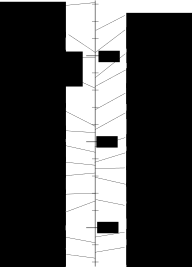
\includegraphics[height=0.8\textheight]{02_Tools/fig/MS_timeline.png}
	\caption{Brief history of mass spectrometry. Most events are described in ref. \citen{Griffiths2008} and at \url{https://en.wikipedia.org/wiki/History_of_mass_spectrometry}. Several later events focus on the coupling of electrochemistry and mass spectrometry: [A], ref. \citen{Hoch1963}; [B], ref. \citen{Bruckenstein1971}; [C], ref. \citen{Wolter1984}; [D], ref. \citen{Wonders2006}; [E], ref. \citen{Henriksen2009}; [F], ref. \citen{Trimarco2015}: [G], Paper \ref{Trimarco2018}.}
	\label{fig:MS_timeline}
\end{figure}

The early development of mass spectrometry was inseparable from the fundamental study of how charged matter behaves under electric and magnetic fields in vacuum, and thus closely tied to many fundamental discoveries in early physics. This includes the discovery of the electron, the discovery of relativistic effects, and the discovery of isotopes. Mass spectrometry has been put to use in an astounding number of applications, including a prominent unsavory one: a modified mass spectrometer was used in one of the purification steps of \ch{^{235}U} for the first atomic bombs (diffusion-based methods and centrifugation have since become much more practical methods of separating isotopes) {\color{red} TOD Manhattan project citation}. Other applications include, for example, trace element analysis (ICP-MS) and protein sequencing (MALDI-TOF).

\begin{figure}[h!]
	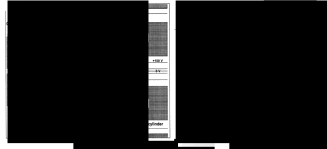
\includegraphics[width=\textwidth]{02_Tools/fig/MS_diagrams.png}
	\caption{Diagram of the components of a quadrupole mass spectrometer (QMS): \textbf{(a)}, electron impact ionization; \textbf{(b)} quadrupole mass separation; and \textbf{(c)},  secondary electron multiplier detection. Adapted from J. Gross, ``Mass Spectrometry'', ref. \citen{Gross2007}. Figure numbers in the image refer to that textbook.}
	\label{fig:MS}
\end{figure}

A mass spectrometer consists of at least three components in a vacuum vacuum chamber\cite{Gross2007}: 

\begin{enumerate}
	\item \textbf{Ion source.} The ion source for the electrochemistry-mass spectrometry (EC-MS) setups described in this Thesis is electron impact ionization (EI, Figure \ref{fig:MS}a). An electron beam is generated by heating up a filament until the high-energy tail of the Fermi distribution of the electrons in the material exceeds the work function of the material. This expels electrons into the vacuum. These electrons are accelerated through a voltage $V$ and pick up an \textit{ionization energy} of $q_\text{el}V$. The ionization energy in this diagram, and throughout this Thesis, is 70 eV. The electrons encounter the molecules to be analyzed (we'll get back to how these molecules got there) in an \textit{ion volume} and impact some of them, imparting a large energy. Many of these impact events result in the expulsion of another electron (or multiple electrons), generating a positively charged ion. Many also result in \textit{fragmentation}, or breaking of the molecules' bonds. It is these \textit{fragments} which are separated and detected by m/z ratio. First they are accelerated from the ion volume to the mass separator.
	
	\item \textbf{Mass separation.} For the EC-MS setups, this is accomplished by a quadrupole (Figure \ref{fig:MS}b). A quadrupole consists of four parallel rods separated by a distance on the order of a centimeter. The rods are connected in two pairs, which are biased by a constant DC bias superimposed on a radio-frequency AC bias. The result is that ions of a specific m/z ratio, which is a function of these two biases, are driven in a stable circular trajectory between the rods and in the plane perpendicular to the rods, whereas ions of other m/z ratios are thrown out by either the AC bias (small ions) or the DC bias (large ions). Ionized fragments enter the four rods with a velocity parallel to the rods, and those with the right m/z ratio fly in neat spirals long enough to make it through. The biases can be changed quickly to scan through a range of m/z ratios (for a \textit{mass spectrum}) or jump between specific m/z ratios of interest to monitor as a function of time (for a \textit{mass-time} measurement). The separation power increases with the length of the quadrupole, and 10 cm is a typical length. 
	
	\item \textbf{Detection.} For the EC-MS setups, this is usually accomplished by a secondary electron multiplier (Figure \ref{fig:MS}c). The ion fragments that make it through the quadrupole hit a detector. In the simplest case, called a \textit{Faraday cup} the detector is just a grounded piece of metal, and the current from the ground, which is equal to the current due to the ions hitting the detector, is measured. However, for higher sensitivity, with a \textit{secondary electron multiplier}, the ions hit the first of a series of charged plates, starting an electron cascade. The current coming out of the last plate, which is orders of magnitude larger than than the ion current hitting the first plate, is recorded as the \textit{mass spectrometer signal}.
\end{enumerate}

Each of the three steps above necessitate high vacuum\cite{Gross2007, PfeifferKnowhow}. (1): The mean free path of electrons should be greater than the distance from the filament to the center of the ion volume, generally a few centimeters,  necessitating a vacuum better than $\sim 10^{-4}$ mbar\cite{Concepts2003}. Furthermore, the lifetime of the filament is decreased significantly at pressures higher than about $\sim 10^{-5}$ mbar. More importantly, the density of ions should be small enough that their mutual repulsion is insignificant compared to the acceleration forces. This begins to be violated when the pressure exceeds $\sim 10^{-6}$ mbar, and the resulting \textit{space-charge effects} cause the signal to no longer respond linearly with the amount of analyte\cite{PfeifferKnowhow, Harris2010}. (2): The mean free path of ions in the vacuum chamber should be significantly greater than the length ($\sim10$ cm) of the quadrupole, necessitating a vacuum better than $\sim 10^{-4}$ mbar\cite{Concepts2003}. (3), The lifetime of the secondary electron multiplier is decreased significantly at pressures higher than about $\sim 10^{-5}$ mbar.

The coupling of mass spectrometry and electrochemistry, motivated at the start of this Chapter, therefore requires an interface letting electrochemical products from a wet, ambient-pressure environment enter a vacuum chamber while maintaining a pressure less than $\sim 10^{-6}$ mbar.

Our version of electrochemistry - mass spectrometry involves making the interface between the liquid electrolyte and the vacuum chamber with a specially fabricated silicon microchip called the membrane chip. This strategy gives a number of unique advantages, and also some disadvantages, which make it ideal for fundamental studies but (in its present implementation) less ideal for high-current \textit{in-operando} studies. For the latter type of study, conventional flow-cell differential electrochemistry - mass spectrometry (DEMS)\cite{Baltruschat2004} retains some advantages. Ours should therefore be thought of as a distinct technique, which we refer to as \textit{chip EC-MS} or just \textit{EC-MS}.

\subsection{Chip EC-MS: working principle}\label{subsec:ECMS}

This Subsection will be brief because the motivation, design principles, and original implementation of Chip EC-MS are described extensively in a fantastic PhD Thesis by Daniel Trimarco (ref. \cite{Trimarco2017_PhD}) and in the article which we wrote together, included in this Thesis as Paper \ref{Trimarco2018}. 


\begin{figure}[h!]
	\centering
	\includegraphics[width=\textwidth]{02_Tools/fig/chip_ECMS_diagram.png}
	\caption{\textbf{(a)} Schematic diagrams of chip-based EC-MS and photographs of the membrane chip, adapted from Paper \ref{Trimarco2018} \textbf{(b-c)} Visual microscopy images of the (a) front of the chip showing the membrane, scale bar = 20$\mu$m and (b) back of the chip showing the capillary through the transparent Pyrex, scale bar = 200$\mu$m.}
	\label{fig:chipECMS}
\end{figure}

Figure \ref{fig:chipECMS} includes schematic diagrams of the key components of chip EC-MS. Membrane chips are fabricated at wafer-scale from semiconductor-on-oxide (SOI) wafers with standard clean-room techniques. Photographs of the front and the back of the chip, are shown in the bottom right corner. The photograph of the front of the chip is colorful due to the diffraction of visible light by the chip's membrane. The membrane consists of thousands of holes with a diameter of 2.5 $\mu$m patterned over a circle 7 mm in diameter by UV lithography. Below the membrane is an empty volume, called the \textit{sampling volume} formed by etching of the SOI's oxide layer. The sampling volume is connected to the back of the chip by four holes formed by deep reactive ion etching (DRIE) from the back. A series of gas channels are formed on the back by UV lithography: a wide carrier gas reservoir channel connecting the carrier gas inlet to the carrier gas outlet (indicated in blue in the chip schematic at the top right of Figure \ref{fig:chipECMS}a, three carrier gas delivery channels (intended to achieve symmetric gas flow - indicated by one green channel in the schematic), and a capillary connecting to the mass spectrometer inlet (red in the schematic). These gas channels are sealed by anodic bonding to a Pyrex glass wafer, such that the finished chip is silicon on the top and glass on the bottom. The holes for the carrier gas inlet, carrier gas outlet, and mass spectrometer inlet are formed in the Pyrex with a \ch{CO2} laser prior to bonding. The chip is mounted on the This membrane chip design is protected by two patents {\todo cite Daniel's patents} and commercialized by Spectro Inlets ApS.

\begin{figure}[h!]
	\centering
	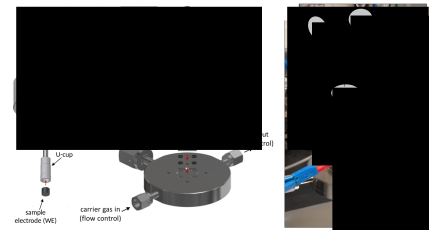
\includegraphics[width=\textwidth]{02_Tools/fig/chipECMS_diagrams_2.png}
	\caption{Diagrams of \textbf{(a)} the cell + working electrode assembly and \textbf{(b)} The cell + chip + interface block assembly. \textbf{(c)} Photo of the setup in use. From Paper \ref{Trimarco2018}}
	\label{fig:chipECMS2}
\end{figure}

The membrane chip is intended as a \textit{window} into what is happening on (or more specifically, what is desorbing from) the surface of an electrochemical sample. This requires the establishment of a three-electrode setup with the working electrode parallel to and close to the membrane. We accomplish this with an \textit{EC-MS cell}, diagrammed on the top-left of Figure \ref{fig:chipECMS}a and in Figure \ref{fig:chipECMS2}a. The cell is most simply described as a piece of polychlorotrifluoroethylene (PCTFE or Kel-F) with holes machined in it. The holes include a cavity through the center for the working electrode assembly. We use the Change-Disk RDE equipment commercially available from Pine Research Instruments for quick and versatile sample exchange. This system uses a PTFE U-cup, which is squeezed slightly between the sample and the cell, to hold the sample in place. The sample can be any 5 mm disk. The distance between the sample and the membrane of the chip, the \textit{working distance}, is defined by a Teflon spacer, and is 100 $\mu$m throughout this Thesis. The volume between the surface of the working electrode and the membrane chip is called the \textit{working volume}. The concentric 7 mm membrane and 5 mm membrane give rise to a 1 mm x 100 $\mu$m \textit{edge volume}. The high aspect ratio of this edge volume ensures that little to no analyte produced at the electrode is lost by lateral diffusion. 

The internal volume of the cell is connected via channels in the EC-MS cell to threaded openings at the top, which are generally fitted with Luer adapters for interfacing with liquid pathway components. In two of these, we place a piece of custom-made glassware with a Luer tip, a ceramic frit to prevent convection, and a large cylindrical volume above. These glassware house the reference and counter electrodes. The other two openings are then used as electrolyte inlet and outlet. To avoid bubbles, the cell must be filled with electrolyte through the inlet before the reference and counter glassware are inserted.

Electrolyte is not typically flowed during experiments. The cell is thus a \textit{stagnant thin-layer} cell. The working volume functions as a perfect diffusion layer, making it relatively easy to model mass-transport in the system.  This mass-transport model was first presented in my Master's Thesis\cite{Scott2016_MSc}, and later refined and verified experimentally in Paper \ref{Trimarco2018}. I will not redevelop the model here, but I will use its results from time to time throughout this Thesis.

As mentioned at the start of this chapter, chip EC-MS has two great advantages over conventional systems for fundamental studies in electrocatalysis: (1) Extremely high sensitivity. This is possible because the chip membrane serves as an equilibration step, letting volatile gases evaporate without sucking in solvent. The very low solvent flux means that no differential pumping stage is necessary, unlike DEMS. Furthermore, the low solvent flux is the reason it is possible to run long experiments without flowing electrolyte. Together, this means that \textit{every molecule of volatile product produced on the electrode will make it to the mass spectrometer} (2) The ability to quickly dose and purge reactant gases. This is possible because the equilibrium of the gas-liquid interface at the chip's membrane works both ways: dissolved gases are released, and the gas fed into the chip saturates the working volume.

\subsection{Chip EC-MS: implementation}\label{subsec:setups}

In practice, an external system for vacuum and gas handling is needed to realize the advantages of high sensitivity and quick reactant gas dosing and purging made possible by chip EC-MS. This Subsection describes two such vacuum systems that I worked on during this PhD project. The vast majority of my work was done on the so-called ``Sniffer setup'' at DTU. During my external stay in professor Zhenhai Wen's group at the Chinese Academy of Sciences (CAS) in Fuzhou, I designed a more compact version, which became the EC-MS 200A. In the spirit of making this Thesis useful to my colleagues, I will describe the procedures of pumping down the chip and exchanging gases with reference to the valve diagrams.

\textbf{\large The Sniffer Setup at DTU:}
\begin{figure}[h!]
	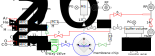
\includegraphics[width=\textwidth]{02_Tools/fig/setup_sniffer.png}
	\caption{Valve diagram of EC-MS setup at DTU. Adapted from Paper \ref{Trimarco2018}. Red: components installed since that publication. Green: The 6-way valve was removed since then as well as the pneumatic valves before the pressure controllers, which were re-purposed. Blue: The interface block, as well as the valve right before it, were replaced to minimize the intervening volume, enabling faster exchange of gases.}
	\label{fig:sniffer}
\end{figure}


\textbf{\large The ECMS-200A in Fuzhou:}

\begin{figure}[h!]
	\centering
	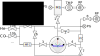
\includegraphics[width=0.75\textwidth]{02_Tools/fig/setup_Fuzhou.png}
	\caption{Valve diagram of EC-MS setup at Fuzhou}
	\label{fig:Fuzhou}
\end{figure}

\textbf{\large Spectro Inlets:}


\subsection{Example experiments: RHE potential measurement and CO stripping}\label{subsec:examples}

\begin{figure}[h!]
	\centering
	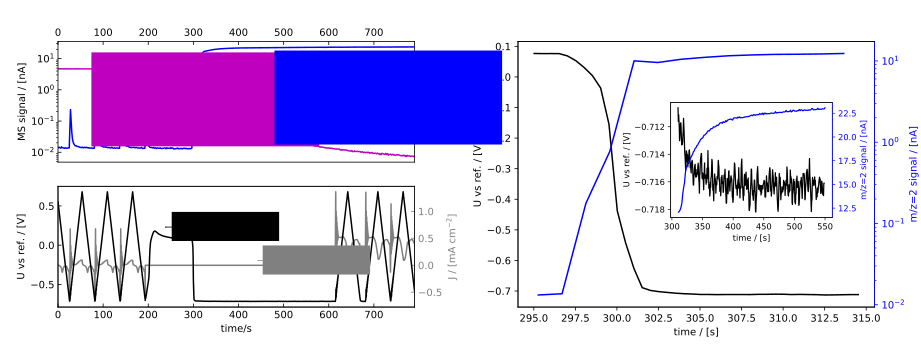
\includegraphics[width=\textwidth]{02_Tools/fig/RHE_calibration.png}
	\caption{RHE calibration experiment using a polycrystalline platinum electrode. \textbf{(a)} EC-MS plot with mass spectrometer signals in the top panel and the concurrent electrochemical data in the lower panel. \textbf{(b)} A zoom-in on the time at which the carrier gas is switched from helium to hydrogen while the electrode is at OCP, showing the electrode potential (black, left y-axis) co-plotted with the m/z=2 signal (blue, right y-axis)}.
	\label{fig:RHE_cal}
\end{figure}

\begin{figure}[h!]
	\centering
	\includegraphics[width=\textwidth]{02_Tools/fig/Trimarco2018_fig03.png}
	\caption{Experiments showing HER, OER, CO oxidation, and CO stripping on Pt. For a detailed discussion, see Paper \ref{Trimarco2018}. \textbf{(a)} and \textbf{(c)} show EC-MS plots and \textbf{(b)} and \textbf{(d)} each show two parts of the respective data set co-plotted against potential. From Paper \ref{Trimarco2018}.}
	\label{fig:fig3}
\end{figure}

\subsection{Disadvantages}\label{subsec:disadvantages}


\begin{figure}[h!]
	\includegraphics[width=\textwidth]{02_Tools/fig/fig07_old.png}
	\caption{Model comparing the sensitivity of chip EC-MS to conventional DEMS via the collection efficiency in a hypothetical flow setup. Adapted from Paper \ref{Trimarco2018}.}
	\label{fig:sensitivity}
\end{figure}

\begin{figure}[h!]
	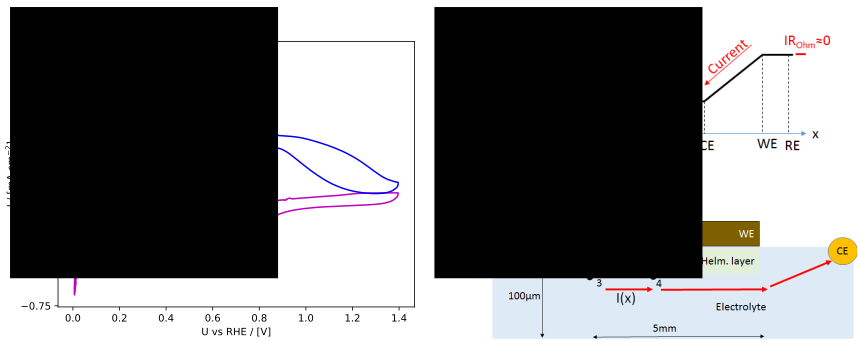
\includegraphics[width=\textwidth]{02_Tools/fig/nonideal_current_distribution.png}
	\caption{\textbf{(a)} CV's in He (magenta) and \ch{H2} from Figure \ref{fig:RHE_cal}. The squiggles are the result of oscillations caused, in part, by electrolytic resistance accross the surface of the sample. \textbf{(b)} Schematic diagrams of electrode connections to the working volume, indicating that while the conventional ohmic resistance is zero, the resistance within the working volume means that the electrochemical potential is not uniform. Adapted from my Master's Thesis\cite{Scott2016_MSc}}.
	\label{fig:current_distribution}
\end{figure}

